% vim:set et sts=2 sw=2 ts=2 tw=72:

Git is a distributed version control system that is used in many
open-source and closed-source projects. Git enables many developers to
write code simultaneously, working on various components known as
branches. Git uses a directed acyclic graph model (DAG) for storing the
necessary information regarding the state of the code at any point in
time. Git refers to nodes of the DAG as commits, not distinguishing
between the code-carrying commits and the structural commits that bring
two branches together. In this paper, we will refer to the individual
commits as being commits, the structural merge commits as merges, and
refereeing to all as repository events.

Between 50k and 70k commits are added to the Linux kernel per version
requiring maintainers of older versions of the kernel to sift through
thousands of commits and merges with tools that are unable to filter and
effectively visualize projects at the scale of the kernel. Older
versions of the kernel are used in embedded systems and mobile phones;
for security purposes, performance needs, and changing hardware
requirements, maintainers must be able to understand the changes being
made in the current version of the kernel in order to produce the
necessary patches for the older versions of the kernel. Current tools
and visualizations are based on the directed acyclic graph (DAG) of the
repository, showing all commits and merges in chronological order by
when the commit was authored, not by when it arrived in the official
Linux repository.

\begin{figure}
  \centering
  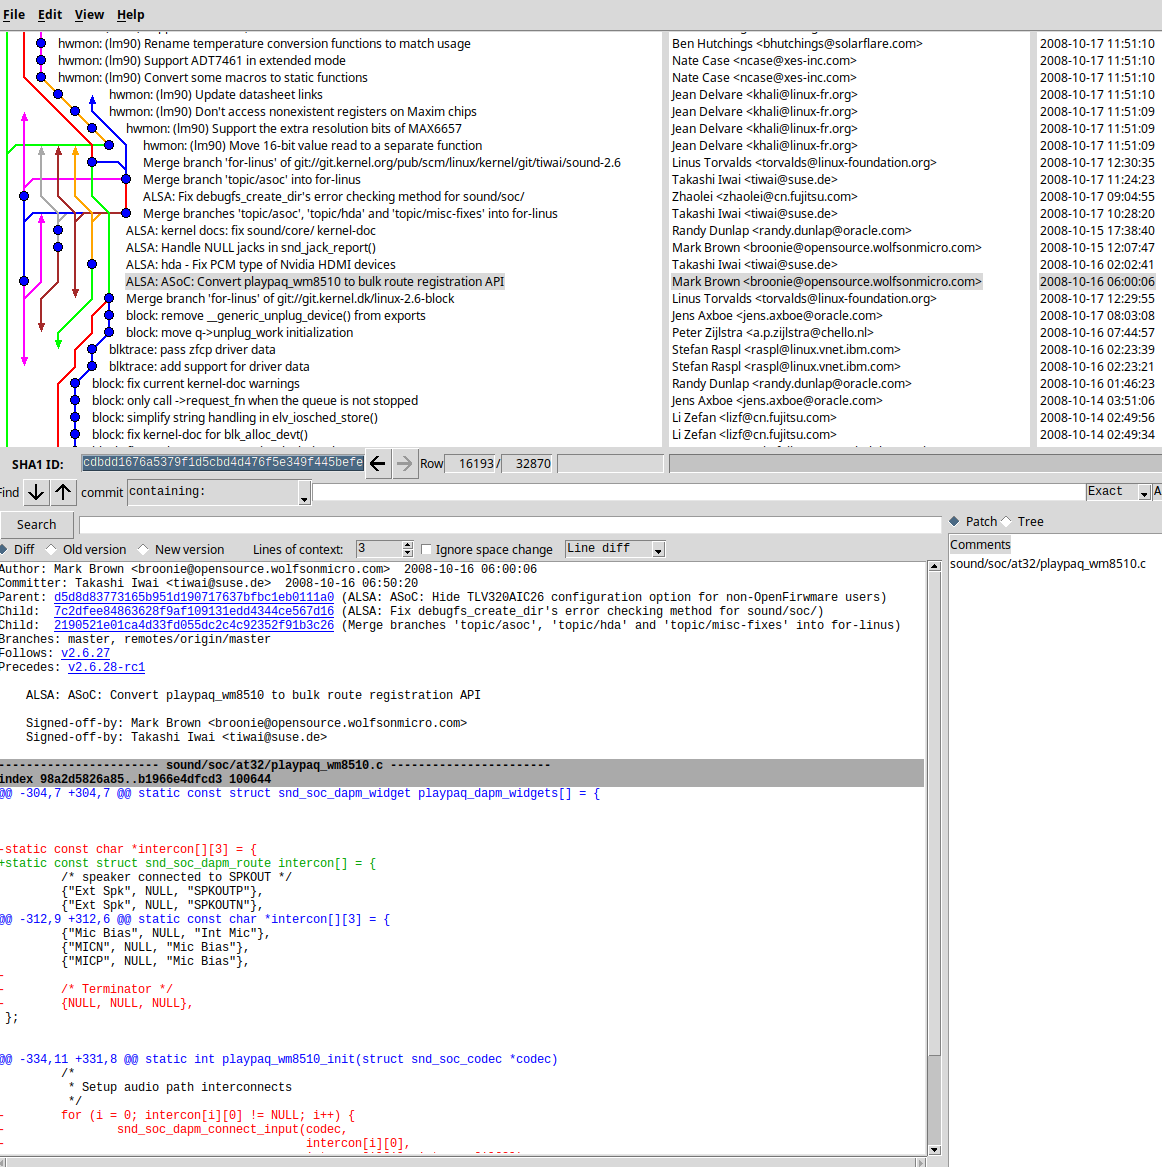
\includegraphics[width=0.8\linewidth]{figures/gitk.png}
  \caption{
    The Gitk interface, centered at commit
    cdbdd1676a5379f1d5cbd4d476f5e349f445befe. The top left pane showing
    the DAG, the top center pane showing the authors, and top right pane
    showing the commit dates. The bottom-left pane shows the full
    commit message and diff of the selected commit, and the bottom-right
    pane shows the list of the files modified by the selected commit.
  }
  \label{fig:gitk}
  %\vspace{-4mm}
\end{figure}

% DAG model

The DAG representation works in smaller projects; it enables users to
see when changes are made, when these changes are merged, how each
branch is interacting, and the point where a branch forks from the
master branch. In large modular projects, like the Linux kernel, the DAG
becomes a mess of merges and commits (Figure~\ref{fig:gitk}) losing its
visual meaning. In some cases, the repository is simply too large for
systems to generate a visualization; repositories stored on GitHub will
have a DAG visualization to show the branches and forks of a
repository, but is unable to display the visualization for projects at
the scale of Linux or even the Git Git
repository(Figure~\ref{fig:gitfail}). Between 60k and 70k new commits
are created for the Linux project every year; according to previous
work\cite{German2015}, a commit takes a median of 30 days from the time
it is authored until it arrives in the official repository. The snapshot
of the kernel tomorrow may be different than the snapshot from today,
containing new commits authored in the past; distinguishing these new
commits from the commits in the snapshot from today is not trivial.

\begin{figure}
  \centering
  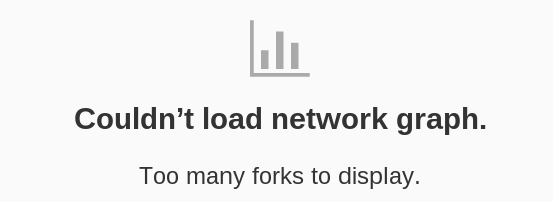
\includegraphics[width=0.8\linewidth]{figures/github_viewer.png}
  \caption{Github is unable to display the DAG of the Linux
    Project due to the size and complexity, which would normally
    show the relationship to other branches and forks.}
  \label{fig:gitfail}
  %\vspace{-2mm}
\end{figure}

% Merge tree model

We propose a new model, built from the DAG, with the purpose of
providing a clearer conceptual image of how a commit is merged, other
commits that are merged with a commit, and a summarization of the entire
group of commits that are merged with a commit. We call our model the
\mt model. The model inverts the DAG, so that reference point from
parent to child instead of from child to parent. This enables the
aggregation of commit metrics at merges. Given a merge, we are able to
recursively traverse the children of the merge, collecting the
statistics at each commit. The commits become the leaves of the tree,
and internal nodes are merges that do not merge into the master branch
of the repository. We terminate the further traversal of an edge under
two conditions; first, if the next event is on the master branch of the
repository, second, if the next event has a shorter path into the master
branch of the repository. As a consequence, commits will always take the
shortest path, in terms of commit time, to the master branch.

A short example: assume the commits represented in
Figure~\ref{fig:repoEvents} show the sequence of events in a repository.
In this case, commits are performed in various repositories and
branches. The DAG representation of the commits is shown in
Figure~\ref{fig:repoDAG}. Notice that the DAG loses information about
the master branch and the repository that the master branch is part of.
The \mt view of this DAG is visible in Figure~\ref{fig:repoTree}.
Note that the direction of the edges of the DAG have been inverted,
instead of pointing from the child to the ancestors, it points from the
ancestor to its successors, forming a path to the master branch. Also
note that the DAG has been simplified, showing only a single edge on the
path to master for any commit.

\begin{figure}[htbp]
  \centering
  \begin{tikzpicture}[auto, on grid, semithick, state/.style={circle, text=black}]
    \foreach \x in {0, 1, 2, 3, 4, 5, 6, 7}
    \draw[shift={(\x + 0.5, -0.5)}, color=black] (0cm, 4cm) -- (0pt, -0.2cm);

    \node[state, draw=chartblue] (1) {1};
    \node[state, draw=chartyellow, above right= of 1] (2) {2};
    \node[state, draw=chartmagenta, above right= 2cm and 1cm of 2] (3) {3};
    \node[state, draw=chartblue, right= 2cm of 1] (4) {4};
    \node[state, draw=chartyellow, above right=of 4] (5) {5};
    \node[state, draw=chartred, above right=of 5] (6) {6};
    \node[state, draw=chartyellow, right=of 5] (7) {7};
    \node[state, draw=chartmagenta, above right= 2cm and 1cm of 7](8) {8};
    \node[state, draw=chartyellow, right= 2cm of 7] (9) {9};
    \node[state, draw=chartyellow, right=of 9] (10) {10};
    \node[state, draw=chartblue, below right=of 9] (11) {11};
    \node[state, draw=chartblue, below right=of 10] (12) {12};

    \draw (12) edge[-stealth] (11) edge[chartyellow, -stealth] (10);
    \draw (11) edge[-stealth] (4) edge[chartyellow, -stealth] (9);
    \draw (10) edge[chartyellow, -stealth] (9);
    \draw (9) edge[chartmagenta, -stealth] (8) edge[chartred, -stealth] (6)
              edge[chartyellow, -stealth] (7);
    \draw (8) edge[chartmagenta, -stealth] (7);
    \draw (7) edge[chartyellow, -stealth] (5);
    \draw (6) edge[chartred, -stealth] (5);
    \draw (5) edge[chartmagenta, -stealth] (3) edge[chartyellow,-stealth] (2)
              edge[chartyellow, -stealth] (4);
    \draw (4) edge[-stealth] (1);
    \draw (3) edge[chartmagenta, -stealth] (2);
    \draw (2) edge[chartyellow, -stealth] (1);

    \node [draw=chartblue, below = 1.5cm of 1] (l1) {Master};
    \node [draw=chartyellow, right = 1.5cm of l1] (l2) {Repo A};
    \node [draw=chartred, right = 2.5cm of l2] (l3) {Branch of Repo A};
    \node [draw=chartmagenta, right= 2.5cm of l3] (l4) {Repo B};

        \foreach \x in {0, 1, 2, 3, 4, 5, 6, 7, 8}
    \node[shift={(\x, -0.6)}, color=black] {$t_\x$};
  \end{tikzpicture}
  \caption{Example of a sequence of events performed in different
    repositories. The horizontal axis represents time. Each horizontal
    section represents a different branch and/or repository. Each commit
    points to its ancestor.}
  \label{fig:repoEvents}
%\vspace{-3mm}
\end{figure}

\begin{figure}[htbp]
  \centering
  \begin{tikzpicture}[auto, on grid, semithick, state/.style={circle, text=black}]
    \node[state] (1) {1};
    \node[state, above right= of 1] (2) {2};
    \node[state, above right= 2cm and 1cm of 2] (3) {3};
    \node[state, right= 2cm of 1] (4) {4};
    \node[state, above right=of 4] (5) {5};
    \node[state, above right=of 5] (6) {6};
    \node[state, right=of 5] (7) {7};
    \node[state, above right= 2cm and 1cm of 7](8) {8};
    \node[state, right= 2cm of 7] (9) {9};
    \node[state, right=of 9] (10) {10};
    \node[state, below right=of 9] (11) {11};
    \node[state, below right=of 10] (12) {12};

    \draw (12) edge[-stealth] (11) edge[-stealth] (10);
    \draw (11) edge[-stealth] (4) edge[-stealth] (9);
    \draw (10) edge[-stealth] (9);
    \draw (9) edge[-stealth] (8) edge[-stealth] (6)
              edge[-stealth] (7);
    \draw (8) edge[-stealth] (7);
    \draw (7) edge[-stealth] (5);
    \draw (6) edge[-stealth] (5);
    \draw (5) edge[-stealth] (3) edge[-stealth] (2)
              edge[-stealth] (4);
    \draw (4) edge[-stealth] (1);
    \draw (3) edge[-stealth] (2);
    \draw (2) edge[-stealth] (1);
  \end{tikzpicture}
  \caption{DAG representation of the commits represented in
    Figure~\ref{fig:repoEvents}. The DAG does not maintain the
    information about which repository a commit comes from. Furthermore,
    the DAG does not distinguish the master branch from other branches.}
  \label{fig:repoDAG}
\vspace{-3mm}
\end{figure}

\begin{figure}[htbp]
  \centering
  \begin{tikzpicture}[auto, on grid, semithick, state/.style={circle, text=black}]

    \draw[chartblue]
      (-0.5, -0.5) -- (8.5, -0.5) -- (8.5, 0.5) -- (-0.5, 0.5) -- (-0.5, -0.5);

    \node[state, draw=chartblue] (1) {1};
    \node[state, draw=chartyellow, above right= of 1] (2) {2};
    \node[state, draw=chartmagenta, above right= 2cm and 1cm of 2] (3) {3};
    \node[state, draw=chartblue, right= 2cm of 1] (4) {4};
    \node[state, draw=chartyellow, above right=of 4] (5) {5};
    \node[state, draw=chartred, above right=of 5] (6) {6};
    \node[state, draw=chartyellow, right=of 5] (7) {7};
    \node[state, draw=chartmagenta, above right= 2cm and 1cm of 7](8) {8};
    \node[state, draw=chartyellow, right= 2cm of 7] (9) {9};
    \node[state, draw=chartyellow, right=of 9] (10) {10};
    \node[state, draw=chartblue, below right=of 9] (11) {11};
    \node[state, draw=chartblue, below right=of 10] (12) {12};

    \draw (2) edge[chartyellow, -stealth] (5)
          (3) edge[chartmagenta, -stealth](5)
          (5) edge[chartyellow, -stealth] (7)
          (7) edge[chartyellow, -stealth] (9)
          (6) edge[chartred, -stealth] (9)
          (8) edge[chartmagenta, -stealth] (9)
          (9) edge[chartyellow, -stealth] (11)
          (10) edge[chartyellow, -stealth] (12);


  \end{tikzpicture}
  \caption{\mt view of the commits  represented in
    Figure~\ref{fig:repoEvents} showing the path they followed to reach
    the master branch. In this model the successors of each commit
    represents the path followed by that commit to reach the master
    branch.}
  \label{fig:repoTree}
\vspace{-3mm}
\end{figure}

Computing the \mt from a DAG for any repository may not be
possible; however, certain features of the development process of Linux
make it feasible to compute the \mt for the Linux repository.
First, the master branch of Linux is maintained by Linus Torvalds, and
only Linus has write access to it. We have verified this assertion in
previous research~\cite{German2015}. We have developed a heuristic that
is presented in Algorithm~\ref{fig:alg}. In short, the algorithm first
identifies the commits made directly to the master branch; whereafter it
recursively determines the shortest path (in terms of time), using the
DAG, from each commit to the master branch using the inverted DAG.

\begin{algorithm}
        \caption{Computing the \mt from Linux Git's DAG}\label{fig:alg}
        \label{alg:original}
        \begin{algorithmic}
                \Function{ComputeMergeTree}{DAG}: tree
                \State {\# Compute the tree from the DAG of Linux repository.}
                \State {\# Returns $Tree$, a graph containing every commit }
                \State {\# in DAG with the path it followed to master.}

                \State $head \gets \textit{Head of master of git repository}$
                \State $master \gets \textit{traverse DAG from head using }$
                \State \quad\quad\quad\quad $\textit{first ancestor until reaching root}$
                \State $nodes(Tree) \gets nodes(DAG)$
                \State \Function{distance2Master}{cid} : seconds
                \State {\# Helper function}
                \State {\# Recursively compute shortest distance to master}
                \State {\# setting cid's successor (next) in its way to master.}
                \State {\# This function should be memoized. Otherwise it}
                \State {\# would run in exponential time.}
                \If {\textit{cid in master}}
                \State \Return 0
                \EndIf
                \State    $d \gets 	\infty$
                \State {\# Traverse the inverted DAG}
                \For{$c \in children(cid, DAG)$}
                \If {$c \in master$}
                \State $d_1 \gets commitTime(c)-commitTime(cid)$
                \Else
                \State {$d_1 \gets distance2Master(c)$}
                \EndIf
                \If {$d_1 < d $}
                \State $next \gets c$
                \State  $d \gets d_1$
                \EndIf
                \EndFor
                \State {\# $c$ is the commit that follows $cid$}
                \State {\# in its way to master}
                \State add edge $(cid, next)$ to $Tree$
                \State \Return $d$
                \EndFunction

                \State {\# Compute the distance for each commit}
                \State {\# discarding result}
                \For{$c \in nodes(DAG)$}
                \State $distance2Master(c)$
                \EndFor
                \State \Return $Tree$
                \EndFunction
        \end{algorithmic}
\end{algorithm}

We evaluate the performance of the heuristic using the merge log made by
Linus Torvalds, the original creator of Linux, and primary merger of all
other repository events into the master branch of the repository. In
Figure~\ref{fig:sampleMerge}, we see an example of the merge log.

\begin{figure}[htbp]
  \centering
  {\fontsize{7}{9}
    \begin{verbatim}
Merge: 8cbd84f fd8aa2c
Author: Linus Torvalds <torvalds@linux-foundation.org>
Date:   Tue Aug 10 15:38:19 2010 -0700

Merge branch 'for-linus' of git://neil.brown.name/md

* 'for-linus' of git://neil.brown.name/md: (24 commits)
md: clean up do_md_stop
[... edited for the sake of space]
md: split out md_rdev_init
md: be more careful setting MD_CHANGE_CLEAN
md/raid5: ensure we create a unique name for kmem_cache...
...
    \end{verbatim}}\vspace{-5mm}
  \caption{Example of how merges record a subset of commits being
    merged. The commit only shows the first 20 one-line summaries
    messages for the 24 non-merge commits it merged. The ending
    ``\ldots'' is part of the log and represents that other
    commits were merged.}
  \label{fig:sampleMerge}
\end{figure}

We use this information to evaluate the accuracy of the \mt model
extracted from the DAG\@. The method we followed started with the
extraction of the commit history up to July 20, 2016. We computed the
merge tree of every commit until then. Since Linus Torvalds mostly does
merging directly into master, we assumed that every merge by him is the
root of a \mt. As described above, the log of a merge-commit usually
contains the number of commits in the merge the first 20 summaries of
commits being merged. We extracted merges by Linus Torvalds using the
command \mycode{log --merges --author='Torvalds} and compared the number
of commits according to the log with the number of commits in the  \mt
rooted in this commit. We also used the summaries of the commits found
in the merge (not necessarily all---see above) to make sure those
commits were in their corresponding merge tree. For example, for the
merge in Figure~\ref{fig:sampleMerge} we would expect that the merge
tree rooted at \mycode{8cbd84f} contains 24 commits, and the one-line
summaries corresponds to commits in that \mt. We also inspected those
with differences to make sure they were true errors.  The results can be
summarized as follows:

\begin{itemize}

  \item

    Five merges were false-errors because their logs did not contain
    accurate information (were probably edited by hand). For example in
    \mycode{42a579a0f\ldots} one commit summary was missing (the line was
    empty), in \mycode {c55d267\ldots} the summaries were reordered.

  \item

    The heuristic correctly identified that 79 of Linus merges (between
    Jun 7, 2014 and Jun 2, 2014) were made to a branch (not master).
    This branch was merged at \mycode{3f17ea6d\ldots} which contained 6809
    commits.

  \item

    The heuristic worked perfectly until Sept 4, 2007, the earliest date
    that it could be verified.  Before this date, and until Dec 12,
    2006, merges did not include a summary of the commits they included,
    hence making it impossible to verify; during this period, however,
    we correctly identified the merges by Linus into master.

  \item

    Before Dec. 12, 2006 (1542 merges) our heuristic breaks due to the
    presence of a \textit{foxtrot} commit (\mycode{c436688\ldots}),
    which confounded the true master branch of a repository (see
    \url{http://bit-booster.blogspot.ca/2016/02/no-foxtrots-allowed.html}
    for a description of the issue).

\end{itemize}

In summary, of the merges after Sept. 4, 2007, our heuristic was correct
in 100\% of the 16,680 commits. It failed in 1,542 commits before Dec.
12, 2006 and in 836 it appears to be correct (Dec 7, 2006 to Sept 4,
2007).

% Evaluation

In order to determine the effectiveness of the merge-tree model on
comprehension and summarization of git repositories, we conducted a
controlled user study on 12 participants. The user study is a
mixed-methods study, with focus on the quantitative aspects in order to
capture how effective the \mt model, if it is, at improving the
correctness, accuracy, and time performance metrics of users when
performing summarization tasks. We use the qualitative questions as a
means of determine the preference of the participants, and what aspects
they preferred from each tool.

We formulate three research questions that this study is attempting to
answer;

\begin{RQ}
  \item

    Is the DAG able to provide users with an understanding of the events
    in a repository?

  \item

    Do \mt make a difference in the ability to summarize basic
    aggregated information?

  \item

    Do users prefer the \mt model to the DAG for summarization and
    comprehension tasks?

\end{RQ}

% Implementation

We implement a tool, \tool, to test and verify the capabilities of the
\mt model. \tool provides search, summarization, and
visualization using the \mt model.

We provide users with search-based navigation. The search engine takes a
plain text query from the user and returns results based on similarity
to the query. The engine weighs various fields, including the commit
log, the author name, the commit hash, and the dates that the commit was
authored and committed. The results are aggregated by the \mt
with a link to the root at the top, and the repository events that match
the search query in a table below.  An example of a single \mt is shown
in Figure~\ref{fig:linvis_search_results}.

\begin{figure}[htpb]
  \centering
  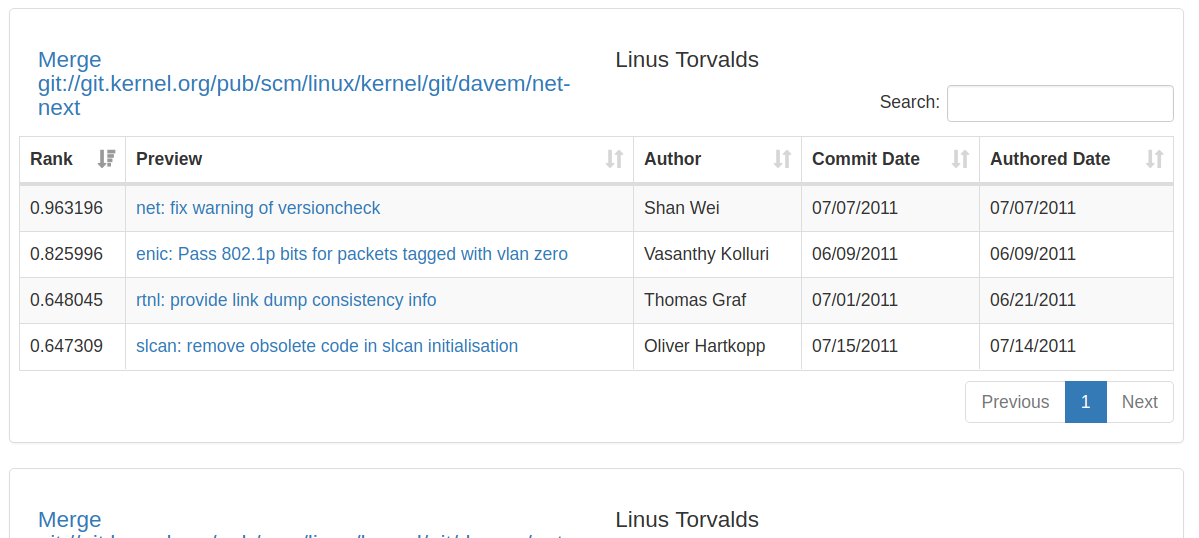
\includegraphics[width=1.0\linewidth]{figures/linvis/search_results.png}
  \caption{\tool search results for `net-next 2011', showing a single
    \mt group.}
  \label{fig:linvis_search_results}
\end{figure}

\tool uses seven tabs to show the information and visualizations for a
selected commit or merge. The message tab shows the full commit log
message. This does not include the diff. The files tab shows an
aggregated table of all files that were modified in a merge. It includes
metrics like the number of lines added, lines removed, total lines
modified, and the delta, summed across all commits in the merge tree
that modify this file. A small details drop-down button allows a user to
see exactly which commit makes the changes, as shown in
Figure~\ref{fig:linvis_files}. If the current repository event being
viewed is a commit, the aggregate views will only show modifications
made by the commit. The modules tab shows the modules modified in the
merge tree. Like the files tab, the modules tab uses a table to show the
name of the module, the number of commits that are in the merge tree
that work with the module, and a details button to provide the links to
those commits.

\begin{figure}[htpb]
  \centering
  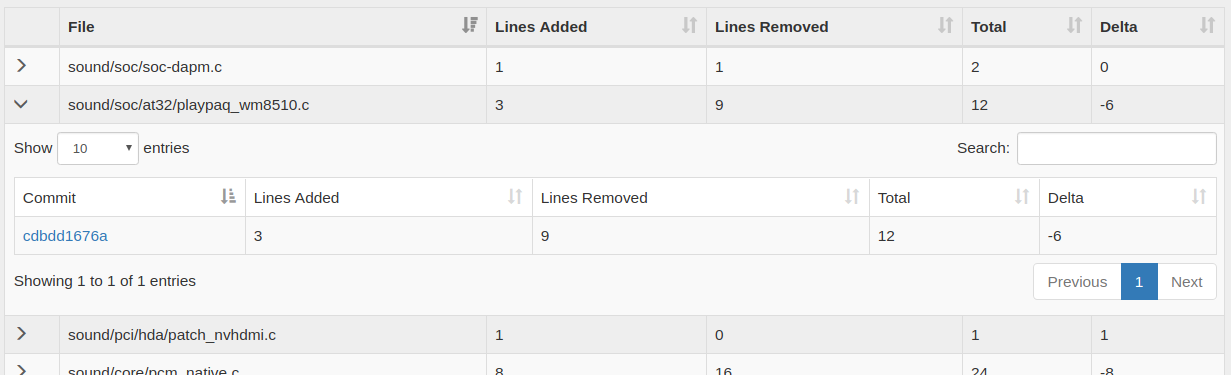
\includegraphics[width=1.0\linewidth]{figures/linvis/linvis_files.png}
  \caption{Table showing the modified files in a merge, with the second
  entry expanded to show the commit that makes the changes.}
  \label{fig:linvis_files}
\end{figure}

The authorship tab is very similar to the files tab, but shows the
authorship information. It shows the sum of the number of lines added,
removed, modified, and the delta within the \mt. It also shows
the number of files that were modified by the author. The details tab is
organized slightly differently. Instead of organizing these results by
commit, the details are organized by file, showing which files were
modified by the author in this \mt (Figure~\ref{fig:linvis_authors}).

\begin{figure}[htpb]
  \centering
  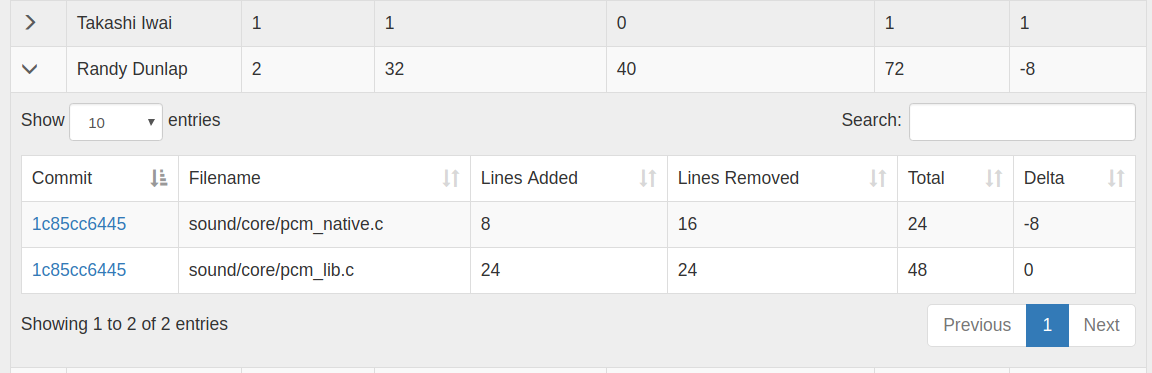
\includegraphics[width=1.0\linewidth]{figures/linvis/linvis_authors.png}
  \caption{Table showing the authors who made changes in a merge. The
    entry for Randy Dunlap is expanded, showing the modifications to
    each file that were made by Randy.}
  \label{fig:linvis_authors}
\end{figure}

\tool implements three visualizations, a list tree, pack tree, and
Reingold-Tilford tree. The list tree is a series of indented textual
lists that can be easily searched with the built-in search in most
web-browsers. The list tree is rooted at the current event, if the event
is a commit, only that commit will be shown; conversely, if the selected
event is the root, the entire merge tree will be shown. The Pack-Tree or
Bubble tree, uses a set-based approach for showing the parent
relationship. The root node aggregates all of the events within the \mt
into the master branch. Thus, the root is the superset of all the other
nodes in the tree. The commits are shown as individual white circles,
containing no other events, as these are the leaves. This is shown in
Figure~\ref{fig:linvis_pack}. The selected event will be shown in bright
orange, commits in white, and merges in shades of blue. Darker shades of
blue indicate that the merge is deeper in the tree.

\begin{figure}[htpb]
  \centering
  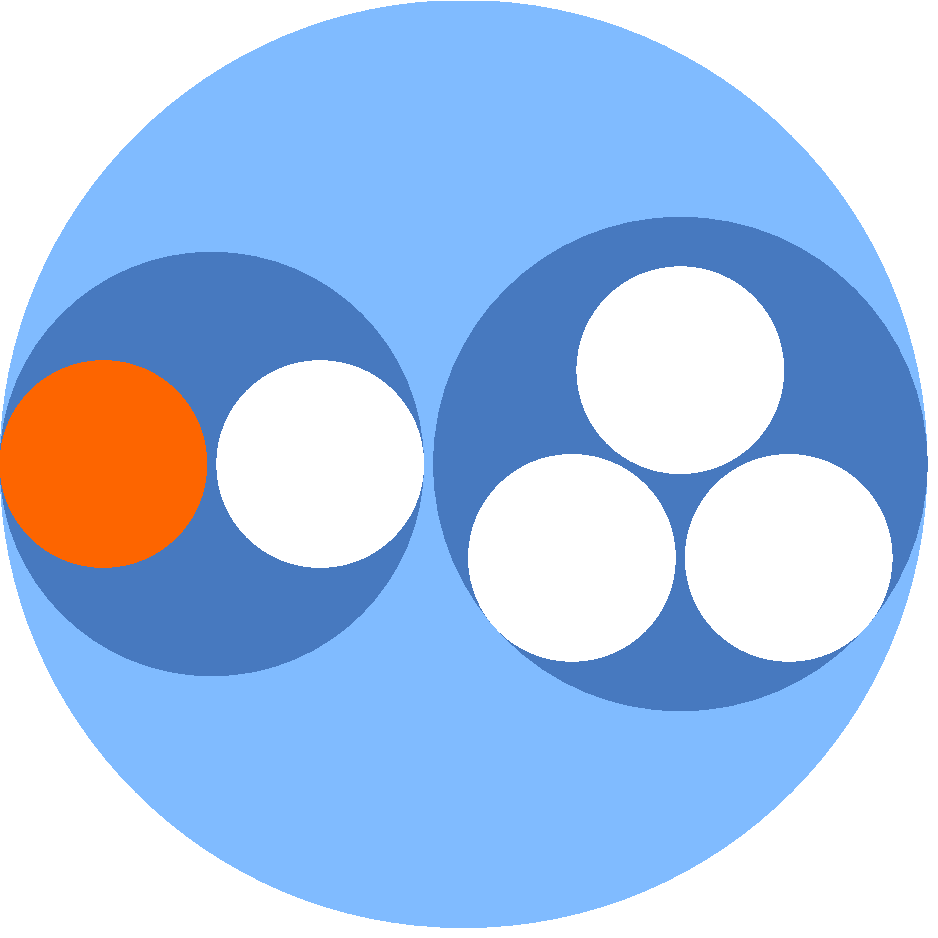
\includegraphics[width=0.8\linewidth]{figures/linvis/linvis_bubble.pdf}
  \caption{The pack tree visualization for a selected commit, shown in
    orange.}
  \label{fig:linvis_pack}
\end{figure}

The Reingold-Tilford tree is the classic tree visualization, with the
root at the top, leaves at the bottom, and the edges between them
showing the parent relationship. An example of the Reingold-Tilford tree
visualization is shown in Figure~\ref{fig:commit_1} and
Figure~\ref{fig:commit_2}.

